\documentclass[10pt,a4paper,twoside, twocolumn]{report}
%% Lots of packages !
\usepackage{etex}

%% Francisation
\usepackage[francais]{babel}
\usepackage[T1]{fontenc}
\usepackage[utf8]{inputenc}
%\usepackage{textcomp}

%% Réglages généraux
\usepackage[left=1.5cm,right=1.5cm,top=2cm,bottom=2cm]{geometry}
\usepackage{fancyhdr}
\usepackage{setspace}
\usepackage{lscape}
%\usepackage{multicol}
\usepackage{makeidx}
\usepackage[clearempty]{titlesec}
\usepackage{cite}

%% Packages pour le texte
\usepackage{pifont}
\usepackage{eurosym}
\usepackage{soul}
\usepackage[normalem]{ulem}
\usepackage{fancybox}
\usepackage{boxedminipage}
\usepackage{enumerate}
\usepackage{verbatim}
\usepackage{moreverb}
\usepackage{listings}
\usepackage[table]{xcolor}

%% Packages pour les tableaux
\usepackage{array}
\usepackage{multirow}
\usepackage{tabularx}
\usepackage{longtable}

%% Packages pour les dessins
\usepackage{graphicx}
\usepackage{wrapfig}
%\usepackage{picins}
\usepackage{picinpar}
\usepackage{epic}
\usepackage{eepic}
\usepackage{tikz}
\usepackage{afterpage}
\usepackage{rotating}
\usepackage{float}
\usepackage{caption}

%% Packages pour les maths
\usepackage{amsmath}
\usepackage{amssymb}
\usepackage{dsfont}
\usepackage{mathrsfs}
\usepackage{bussproofs}
\usepackage[thmmarks,amsmath]{ntheorem}

%% Création de nouvelles commandes
%\usepackage{calc}
\usepackage{ifthen}
\usepackage{xspace}



\usepackage{url}
\usepackage{hyperref}
\usepackage{todonotes}
\usepackage{subcaption}
\usepackage[french,ruled,vlined,linesnumbered,algochapter,dotocloa]{algorithm2e}
\usepackage{MnSymbol}

\usepackage{chngcntr}

\usepackage{standalone}
\usepackage{import}



\frenchbsetup{StandardEnumerateEnv=true}

%% =======================================================================

\fancypagestyle{empty}{%
  \fancyhf{}
  \fancyhead[L]{}
  \fancyhead[C]{}
  \fancyhead[R]{}
  \fancyfoot[L]{}
  \fancyfoot[C]{}
  \fancyfoot[R]{}
}
\fancypagestyle{basicstyle}{
	\fancyhf{}	
	\fancyhead[L]{}
	\fancyhead[C]{Rendu réaliste et temps réel pour la réalité augmentée}
	\fancyhead[R]{}
	\fancyfoot[L]{hadrien.croubois@ens-lyon.fr}
	\fancyfoot[C]{--~\thepage~--}
	\fancyfoot[R]{}
}
\pagestyle{basicstyle}

%% =======================================================================

\titleformat{\section}[frame]
{\normalfont}
{\filright \footnotesize \enspace Partie \thesection\enspace}
{6pt}
{\bfseries\filcenter}
	
\titleformat{\subsection}[frame]
{\normalfont}
{\filright \footnotesize \enspace \thesubsection\enspace}
{6pt}
{\filcenter}

\titleformat{\subsubsection}
{\titlerule \vspace{.8ex} \normalfont\itshape}
{\thesubsubsection}
{.5em}
{}

\titleformat{\chapter}[display]
{\normalfont\bfseries\filcenter}
{}
{1ex}
{\titlerule[2pt] \vspace{2ex} \LARGE}
[\vspace{1ex} {\titlerule[2pt]}]

\parindent=10pt
\DeclareUnicodeCharacter{00A0}{~}

%% =======================================================================



\newcommand{\HRule}{\rule{\linewidth}{0.5mm}}
\newcommand{\Hs}{\operatorname{HS}}




\floatstyle{ruled}
\restylefloat{figure}
\restylefloat{table}
\newfloat{code}{!h}{locode}{}
\floatname{code}{\textsc{code}}

\addto\captionsfrench{%
  \renewcommand{\listfigurename}{Liste des figures}%
  \renewcommand{\listtablename}{Liste des tableaux}%
  \renewcommand{\listalgorithmcfname}{Liste des algorithmes}%
}
\newcommand{\listofcode}{\listof{code}{Liste des codes}}

\numberwithin{code}{chapter}
\numberwithin{equation}{subsection}
\counterwithout{footnote}{chapter}






\newcommand{\framedgraphics}[2]{%
  \setlength{\fboxsep}{0pt}%
  \setlength{\fboxrule}{1pt}%
  \fbox{\includegraphics[{#1}]{{#2}}}%
}

\newcommand*{\captionsource}[2]{%
  \caption[{#1}]{%
    #1%
    \\\hspace{\linewidth}%
    \textbf{\textsc{Source}} #2%
  }%
}

\newcommand{\footurl}[2][]{\footnote{\textbf{#1}\href{#2}{#2}}}
% \newcommand{\footurl}[2][]{\footnote{\textbf{#1}\url{#2}}}







\newif\iftwocolumn
\twocolumntrue
\usetikzlibrary{3d,arrows, calc, backgrounds, petri, positioning, shadows, shapes}


\tikzset{
	persp/.style={scale=3.0,x={(-0.8cm,-0.4cm)},y={(0.8cm,-0.4cm)}, z={(0cm,1cm)}},
	points/.style={fill=white,draw=black,thick}
	grid/.style={very thin,gray},
	axis/.style={->,ultra thick},
	cube/.style={thick, fill=black!15,opacity=0.5},
	cube hidden/.style={dashed},
	block/.style={
		rectangle, rounded corners,
		draw=black!80,
		fill=black!10, fill opacity=0.5,
		text=black!90, text opacity=1.0,
    text height=1.5ex,
    text depth=.25ex,
    text width=6em,
    text centered
	}
}

\tikzstyle{class}			=[rectangle, rounded corners, draw=black, fill=blue!40, drop shadow, text centered, anchor=north, text=white,    text width=3cm]
\tikzstyle{module}		=[rectangle, rounded corners, draw=black, fill=red!40, 	drop shadow, text centered, anchor=north, text=white,    text width=3cm]
\tikzstyle{component}	=[rectangle, rounded corners, draw=black, fill=green,   drop shadow, text centered, anchor=north, text=black!90, text width=3cm]
\tikzstyle{single}		=[text height=1.5ex, text depth=0.25ex]
\tikzstyle{double}		=[text height=4.0ex, text depth=2.75ex]
\tikzstyle{triple}		=[text height=6.5ex, text depth=5.25ex]
\tikzstyle{quadru}		=[text height=9.0ex, text depth=7.75ex]
\newcommand*{\rootPath}{../}
\standalonetrue

\begin{document}

\chapter{Rendu}

%%=====================================================================

\section{État de l'art}

%%=====================================================================

\section{Éclairage ambiant}

\subsection{De la physique aux mathématiques}
Le calcul de l'énergie reçu en un point de l'objet revient à intégrer le flux lumineux sur l'ensemble des direction visibles.
\begin{equation}
	\mathcal E(p, \vec n)=\frac{1}{\pi}\int_{\mathcal{H}^2(\vec{n})}\mathcal L(p,\vec\omega)\times\vec\omega.\vec n\, \mathrm d\vec\omega
\end{equation}

L'intégrale selon $\int_{\mathcal{H}(\vec n)}\mathrm d\omega$ correspond à une intégrale suivant l'hémisphère visible et pondéré par l'angle solide en supposant qu'il n'y a pas d'occultation. Afin de modéliser les phénomènes d'auto-occultation on devrai utiliser la formule suivante

\begin{equation}
	\mathcal E(p, \vec n)=\frac{1}{\pi}\int_{\mathcal V(p, \vec n )}\mathcal L(p, \vec\omega)\times\vec\omega.\vec n\, \mathrm d\vec\omega
\end{equation}
Ou $\mathcal V(p, \vec n)$ est la restriction de l'hémisphère suivant le vecteur $\vec n$ a l'espace effectivement visible depuis le point $p$ (ce qui renvient à considérer $\mathcal H(\vec n)$ privée des direction correspondants à de l'auto-occultation).

Ici on fait d'abord la supposition que l'éclairement selon une direction $\vec{\omega}$ est indépendant du point considéré. Cette approximation, est nécessaire pour utiliser, sans reconstruction 3D complexe, l'envmap reconstruite dynamiquement.

On obtient donc l'équation
\begin{equation}
	\mathcal E(p, \vec n)=\frac{1}{\pi}\int_{\mathcal V(p, \vec n )}\mathcal L_{glob}(\vec\omega)\times\vec\omega.\vec n\, \mathrm d\vec\omega
\end{equation}

On fait alors la supposition que les phénomènes d'auto-occultation influencent de manière moyenne et globale l'énergie reçu en un point. Cela nous permet de revenir à une intégration sur tout le demi espace $\mathcal H^2(\vec{n})$ en ajoutant simplement un coefficient de $\mathcal P_{\mathcal V}(p)$ valant $1$ en l'absence d'auto-occultation et $0$ pour une auto-occultation totale.

Ce coefficient définit sur la surface de l'objet pourra être pré-calculé et fournit sous forme de texture.\todo{reference}

\begin{align}
	\mathcal P_{\mathcal V}(p)	&= \frac{\int_{\mathcal V(p, \vec n(p))}\vec\omega.\vec n\, \mathrm d\vec\omega}{\int_{\mathcal H(\vec n(p))}\vec\omega.\vec n\, \mathrm d\vec\omega}	\notag\\
															&= \frac{1}{\pi}\int_{\mathcal V(p, \vec n(p))}\vec\omega.\vec n\, \mathrm d\vec\omega \\
\intertext{d'ou}
	\mathcal E(p, \vec n)				&= \frac{\mathcal P_{\mathcal V}(p)}{\pi}\int_{\mathcal H(p, \vec n )}\mathcal L_{glob}(\vec\omega)\times\vec\omega.\vec n\, \mathrm d\vec\omega
\end{align}

Enfin, on fera une dernière approximation suivant la méthode proposé dans \cite{Mcguire} : on considère la fonction $\mathcal L_{glob}$ (décrite par l'envmap) comme constante sur chaque face de l'envmap. Le niveau de mipmap le moins détaillé nous donne en effet une valeur moyenne pour la face considérée.


Si l'on oublie un instants les problèmes d'auto-occultation et que l'on s'intéresse a l'angle solide décrit par une face du cube centrée au point de vue, un rapide calcul permet d'évaluer l'angle solide décrit par une face complètement visible comme étant 
\begin{equation}
	\Omega_F = \iint_{F}\frac{1}{\|\vec\omega\|^3}\, \mathrm d\omega = \frac{2\pi}{3}
\end{equation}

L'angle solide sur une face partiellement visible (selon une demi sphère caractérisée par l'hyperplan de vecteur $\vec n$)est alors défini par
\newcommand{\Hs}{\operatorname{HS}}
\begin{equation}
	\Omega_F(\vec n) = \iint_{F}\frac{\Hs(\vec\omega.\vec n)}{\|\vec\omega\|^3}\, \mathrm d\omega
\end{equation}

Avec $\Hs$ la fonction de $\operatorname{HeavySide}$ definie par :
\begin{align}
	\Hs(x) = \begin{cases} 0 &\text{si } x<0 \\ 1 & \text{si } x\geq 0\end{cases} \notag
\end{align}

La figure~\ref{fig:curve:omega_theta} retrace l'évolution de $\Omega_F(\vec n)$ selon l'angle $\theta$ pour des orientation de $\phi=0$ et $\phi=\frac{\pi}{2}$

\begin{figure}[!ht]\centering
	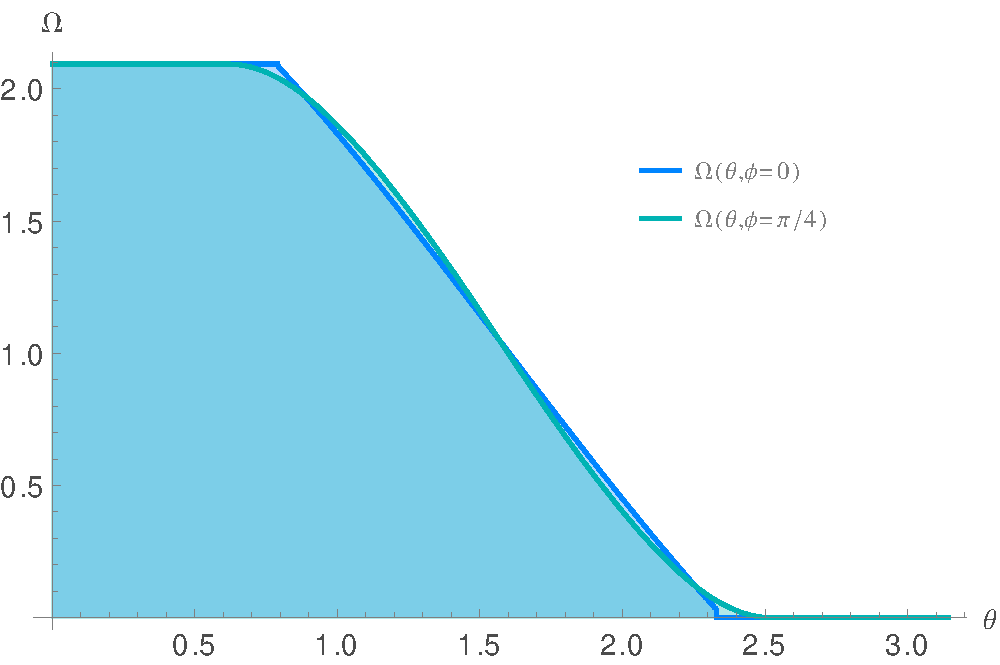
\includegraphics[width=0.4\textwidth]{\rootPath Imgs/graphs/on.pdf}
	\caption{Évolution de $\Omega_F(\vec n)$ selon l'orientation de $\vec n$}
	\label{fig:curve:omega_theta}
\end{figure}

Les poids affectés aux valeurs de chaque face de l'envmap sont donc l'intégration du produit scalaire normalisé $\frac{\vec\omega.\vec n}{\|\vec \omega\|}$ par rapport à l'angle solide sur la face considéré
\begin{align}
	W_F(\vec n)
		&= \iint_{F}\frac{\vec\omega.\vec n}{\|\vec \omega\|}\times\frac{\Hs(\vec\omega.\vec n)}{\|\vec\omega\|^3}\, \mathrm d\omega \notag\\
		&= \iint_{F}\frac{\vec\omega.\vec n\times\Hs(\vec\omega.\vec n)}{\|\vec\omega\|^4}\, \mathrm d\omega
		\label{ref:eq:wintegral}
\end{align}

\begin{figure}[!ht]
	\centering
	\includestandalone[width=0.4\textwidth]{\rootPath Figures/cubemapFacet}
	\caption{Intégration de l'envmap par rapport à une facette}
	\label{fig:tikz:envmapFacet}
\end{figure}

On notera qu'on a bien 
\begin{subequations}
	\begin{align}
					& \sum_{F \in Faces} \Omega(F) 								&=4\pi\\
	\forall \vec n	& \sum_{F \in Faces} \Omega(F,\vec n)	&=2\pi\\	
	\forall \vec n	& \sum_{F \in Faces} W_F(\vec n)			&=\pi	
	\end{align}
\end{subequations}

Dès lors, l'approximation selon laquelle $\mathcal L$ est constante sur chaque face nous donne
\begin{align}
	\mathcal E(p, \vec n)
		& = \frac{\mathcal P_{\mathcal V}(p)}{\pi}\sum_{F \in Faces}\mathcal L_{glob}(\vec F)W_F(\vec n) \notag \\
		& = \frac{\mathcal P_{\mathcal V}(p)}{\pi}\sum_{F \in Faces}\mathcal L_{glob}(\vec F)\iint_{F}\frac{\vec\omega.\vec n\times\Hs(\vec\omega.\vec n)}{\|\vec\omega\|^4}\, \mathrm d\omega
		\label{ref:eq:sumintegral_model}
\end{align}


\subsection{Approximation numérique}


En considérant la face $F_{Z^+}$ on obtient (sans perte de généralité)
\begin{multline}
	W_{F_{Z^+}}(\vec n) = \iint\limits_{[-1;1]^2} \biggl[\frac{(x.\vec n_x+y.\vec n_y + \vec n_z)}{(x^2+y^2+1)^2} \\
	\Hs(x.\vec n_x+y.\vec n_y + \vec n_z)\, \mathrm dx\, \mathrm dy\biggr]
\end{multline}

Le problème est alors de trouver un moyen de calculer, ou au moins d'approcher, la fonction $W_F(\vec n)$. Ce calcul étant par ailleurs fait  en chaque nœud du maillage, il est primordial de le faire en utilisant un minimum de ressource, quitte à évaluer une valeur approchée qui affectera le résultat de manière faible comparativement avec l'approximation faite précédemment et selon laquelle $\mathcal L$ est constante sur chacune faces.

\begin{figure}[!ht]\centering
	\subfloat[$W(\theta)$]{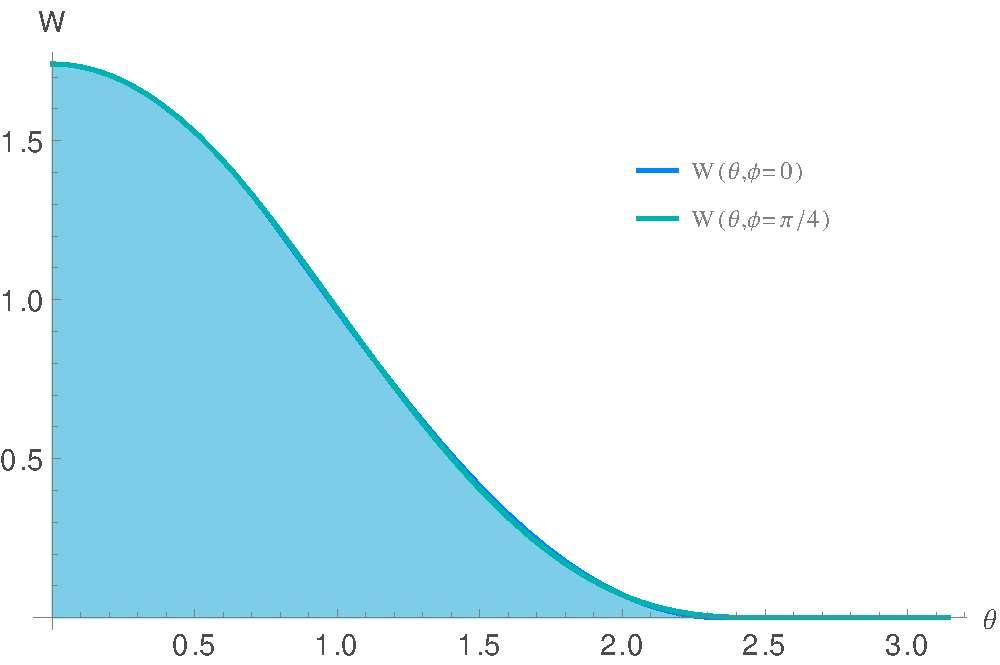
\includegraphics[width=0.4\textwidth]{\rootPath Imgs/graphs/wn.pdf}}
	
	\subfloat[$W(\theta,\phi)$]{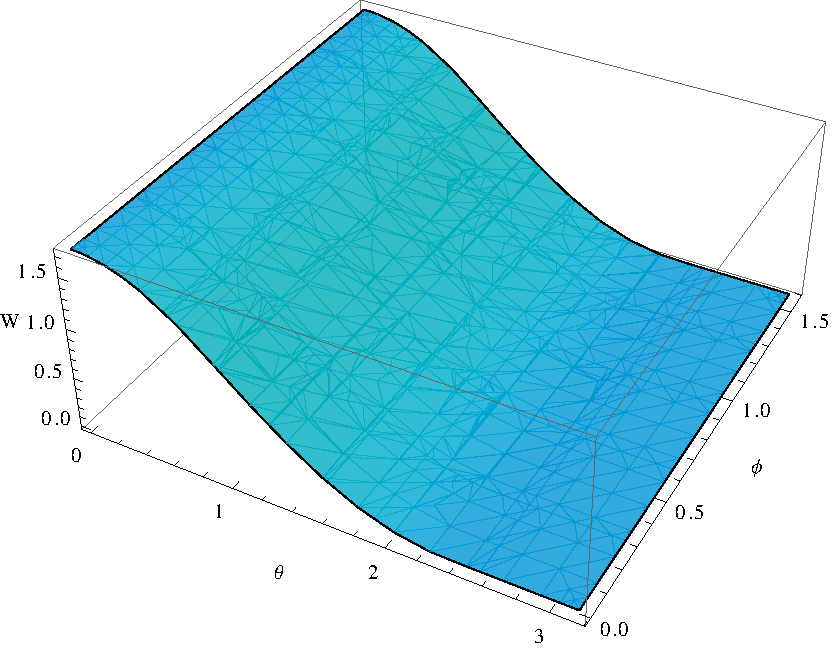
\includegraphics[width=0.4\textwidth]{\rootPath Imgs/graphs/wn3D.pdf}}
	\caption{Évolution de $W_F(\vec n)$ selon l'orientation de $\vec n$ }
	\label{fig:curve:w_theta_phi}
\end{figure}

Comme le montre la figure~\ref{fig:curve:w_theta_phi}, la fonction $W_F$ dépendant principalement de $\theta$ on tentera de l'approximer par une fonction de $\vec n.\vec F = \cos(\theta)$

Une approximation simple est la fonction
\begin{equation}
	approx : \cos(\theta)\mapsto
	\frac{\bigl[\max\left(.75 + \cos(\theta), 0\right)\bigr]^2}{1.75}
\end{equation}
Comme le montre la figure \ref{fig:curve:w_approx}, cette fonction est, malgré sa grande simplicité proche de la fonction $W_F(\vec n)$.

\begin{figure}[!ht]\centering
	\subfloat[$W(\theta)$ et $approx(\cos(\theta))$]{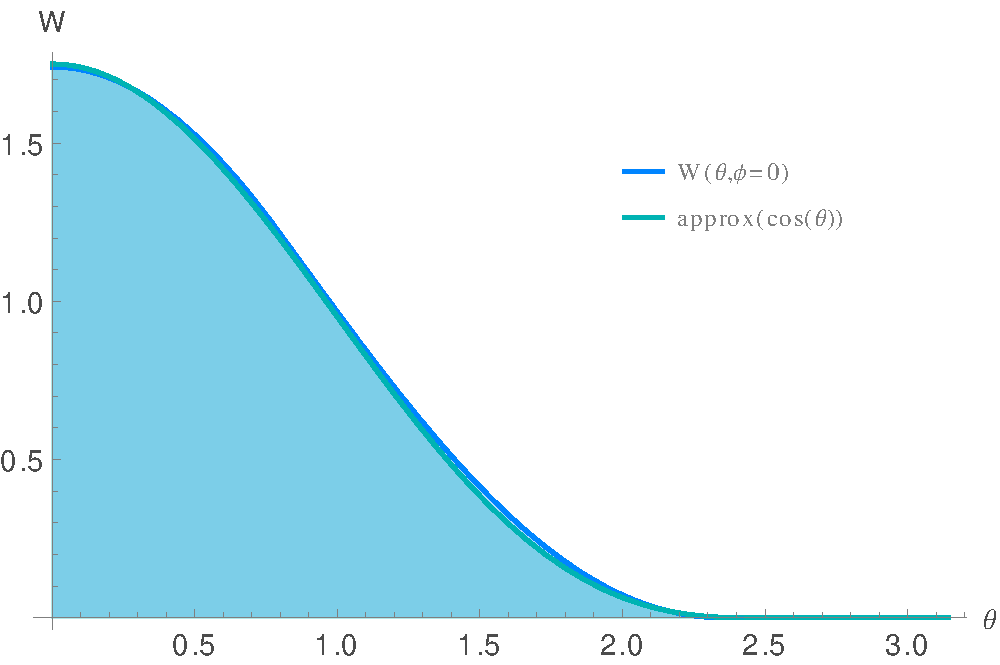
\includegraphics[width=0.4\textwidth]{\rootPath Imgs/graphs/approxw.pdf}}

	\subfloat[$\Delta W$]{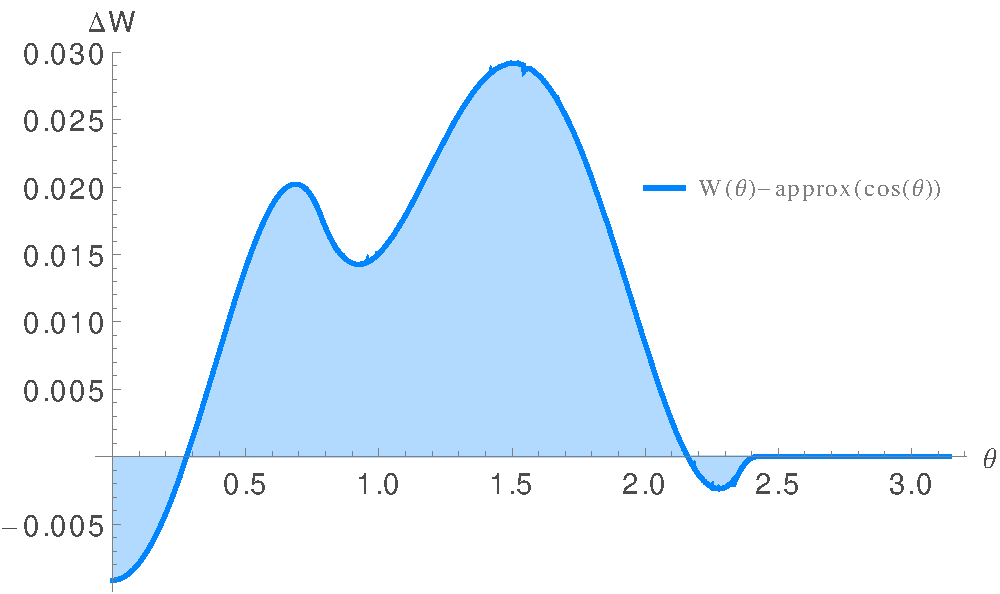
\includegraphics[width=0.4\textwidth]{\rootPath Imgs/graphs/deltaw.pdf}}
	\caption{Comparaison entre $W_F(\vec n)$ et $approx(\cos(\theta))$ }
	\label{fig:curve:w_approx}
\end{figure}


\subsection{Discussion}

La méthode développée ici repose sur l'approximation de la formule~(\ref{ref:eq:sumintegral_model}) et plus particulièrement de l'intégrale présenté dans la formule~(\ref{ref:eq:wintegral}). La complexité de cette intégrale réside dans le domaine effectif d'intégration, conditionné a la fois par la forme carré des faces de l'envmap et la présence d'un terme caractéristique de l'hémisphère visible.

Plusieurs formules ont été étudiée pour des domaines d'intégration hémisphériques ou partiellement hémisphérique ainsi que pour des polygones entièrement visibles \cite{Snyder1996} (ce qui fait disparaître le terme de $\Hs$).

Il aurait été possible d'adapter un modèle polygonale évoqué dans \cite{Snyder1996} mais les polygones sur lesquels il aurait fallu intégrer variant selon les conditions de visibilités il aurait été nécessaire d'effectuer de couteux calculs de géométrie.

L'objectif principal étant ici une grande vitesse d'exécution, l'inexactitude des résultats étant de toute façon largement oubliée au regard des approximations faites précédemment on préféra utiliser une fonction grossièrement approché mais simple à calculer.


%%=====================================================================


\section{Ombrage}

\subsection{Modèle}

Un indice visuel primordiale à la vraisemblance visuel des images produites est la présence d'ombres portées provoquées par l'ajout de l'objet \todo{reference}.

La modélisation de l'impact d'un tel ajout peut théoriquement être calculé qu'en connaissant la géométrie de la scène et la nature des matériaux qui la compose.

On fera ici plusieurs hypothèses dans le but d'obtenir un modèle qui soit calculable en temps réels tout en donnant des résultats vraisemblables.

Le calcul d'ombre douces est alors fait en décomposant l'objet en une hiérarchie de sphère comme présenté dans\cite{Iwanicki} et en sommant les contribution des différentes sphères.

Pour évaluer l'ombre douce projeté par une sphère il suffit alors d'évaluer le manque d'illumination.
On rappel les formules suivantes
\begin{align*}
	\mathcal E_{ambient}(p, \vec n)	&=	\frac{1}{\pi}\int_{\mathcal{H}^2(\vec{n})}\mathcal L_{glob}(\vec\omega)\times\vec\omega.\vec n\, \mathrm d\vec\omega \\
	\mathcal E_{ombre}(p, \vec n)		&=	\mathcal E_{ambient}(p, \vec n) - \frac{1}{\pi}\int_{\mathcal{S}(p)}\mathcal L_{glob}(\vec\omega)\times\vec\omega.\vec n\, \mathrm d\vec\omega
\end{align*}

avec $\mathcal S(p)$ la portion de sphère visible depuis la point considéré.

L'ombre est rendu en assombrissant le pixel associé ce point d'un facteur
\begin{align}
	\mathcal F(p)	&=	\frac{\mathcal E_{ombre}(p, \vec n)}{\mathcal E_{ambient}(p, \vec n)}	\\
								&=	1 - \frac{\int_{\mathcal{S}(p)}\mathcal L_{glob}(\vec\omega)\times\vec\omega.\vec n\, \mathrm d\vec\omega}{\int_{\mathcal{H}^2(\vec{n})}\mathcal L_{glob}(\vec\omega)\times\vec\omega.\vec n\, \mathrm d\vec\omega}	
\end{align}


Les différents niveaux de détail de l'envmap nous permettant d'obtenir des approximations de $L(p,\vec\omega)$ sur $\mathcal S(p)$ et sur $\mathcal{H}^2(\vec{n})$ on peut simplifier la formule en :

\begin{align}
	\mathcal F(p)	&=	1 - \frac{\mathcal L_{glob}(\mathcal{S}(p))}{\mathcal L_{glob}(\mathcal{H}^2(\vec{n}))}\left(\frac{1}{\pi}\int\limits_{\mathcal{S}(p)}\vec\omega.\vec n\, \mathrm d\vec\omega\right)
\end{align}

\begin{figure}[!ht]
	\centering
	\includestandalone[width=0.4\textwidth]{\rootPath Figures/shadows}
	\caption{Obstruction par une sphere}
	\label{fig:tikz:obstruction}
\end{figure}

Le calcul de l'angle solide formé par la sphère, et pondéré par un cosinus est détaillé dans \cite{Snyder1996}. On retiendra que dans notre cas ou la sphère est supposée au dessus du plan sur lequel se projettent les ombres :
\begin{equation}
	\int_{\mathcal{S}(p)}\vec\omega.\vec n\, \mathrm d\vec\omega = \cos(\omega)\sin^2(\alpha)
\end{equation}
avec $\alpha$ le demi angle sous lequel est vu la sphère et $\omega$ l'angle entre la vertical (normale à la surface sur laquelle se projettent les ombres) et la direction de la sphère.

On obtient ainsi :
\begin{align}
	\mathcal F(p)	&=	1 - \cos(\omega)\sin^2(\alpha)\frac{\mathcal L_{glob}(\mathcal{S}(p))}{\mathcal L_{glob}(\mathcal{H}^2(\vec{n}))}
\end{align}


\subsection{Discussion}

La ou il est habituel de segmenter l'environnement pour en extraire une hiérarchie de sources lumineuses, la méthode proposée ici permet d'évaluer des ombres douces à partir de données d'environnement sans étape de segmentation ni calcul de visibilité. 

Un développement intéressant serait de construire une décomposition hiérarchique, potentiellement intégrée dans un octree, et de l'évaluer plus ou moins profondément selon la distance considérée.


%=====================================================================

\section{Reflets spéculaires}

Le calcul de l'éclairage ambiant revient à considérer une BRDF purement lambertienne. Afin d'améliorer le réalisme du rendu il convient d'adopter un modèle de Phong en ajoutant une part d'éclairage spéculaire.

Cet éclairage spéculaire permet de rendre de manière intéressante des surfaces métallique, dans la limite d'un seul reflet. Le modèle adopté ici est par ailleurs isotrope, ce qui ne permet par le rendu de matières comme du métal brossé pour lesquels on retrouve des directions privilégiés.

Dans notre cas l'évaluation du reflet se fait naturellement en calculant la réflexion du rayon incident, donné par la position du point considéré dans l'espace de la camera, relativement à la normale de l'objet dans ce même espace. On accédera ensuite à la valeur d'éclairage directement dans l'envmap.

Une fois de plus on pourra utiliser les différents niveaux de mipmap à notre avantage, la considération du niveau de mipmap revenant la considérer l'angle d'un cône autour de l'axe du reflet. Un tel cône permet ainsi de caractériser la spécularitée de l'objet, cette dernière pouvant varier d'un reflet parfait --miroir-- à un reflet plus diffus --plastique--.
On utilisera également l'ombre projeté calculé précédemment afin de moduler les reflets.

%=====================================================================

\section{Vers un modèles à micro-facettes}

Les modèles employés ici permettent un rendu rapide mais présentes des limitations en terme de qualité. Il serait intéressant, dans l'optique améliorer encore la qualité du rendu, de considérer un modèle à micro-facette. 
Le principes des modèles à micro-facette est de considérer la surface de l'objet comme un ensemble de petites faces orientés selon des normales propres a chacune (micro-normales). La distribution statistique des micro-normales autour de la normale géométrique du maillage (macro-normale) permet de déterminer les mécanismes de réflexion. Parmi les nombreux avantages d'un telle méthode il y a la possibilité de caractériser des surfaces anisotropes par le biais de directions privilégiés dans la distribution de facettes.

L'auto-occultation entre facettes, variable selon le point de vue, permet par ailleurs de calculer une normal intermédiaire entre la normale géométrique et les micro-normales des facette (mézo-normal) qui correspond à l’intégration des micro-normales sur l'ensemble des facette visible\cite{Bruneton2010}\cite{Heitz2013} \todo{figure}. Cette mézo-normale, utilisée à la place de normale géométrique, permet de corriger les reflets sur des surfaces vue sous un angle important.

L’intégration complète d'un tel modèle à été envisagé de la manière suivante :
\begin{enumerate}
	\item Choix d'une distribution de normale (gaussienne) et étude du modèle associé;
	\item Ajout aux objets 3D d'une texture (optionnelle) caractérisant localement la direction privilégiée et la force de l'anisotropie associée;
	\item Évaluer, dans le fragment shader, la distribution de direction reflétées en fonction de l'angle de vue et des caractéristiques stockées dans la texture;
	\item Évaluer la lumière incidente selon la distribution calculée précédemment.
\end{enumerate}

Au delà des calcul complexes, mais heureusement déjà documentées, du premier point\cite{Heitz2013a}, l'évaluation de l'envmap selon des distributions anisotrope nécessite de lourds calculs.
Il serait possible de les réduire fortement via un pré-calcule (convolution) mais dans notre cas le caractère dynamique de l'environnement ne permet pas un telle approche.

Une autre solution est d'approximer cette intégration de l'envmap par le biais d'un filtrage judicieux. \todo{expliquer que textureGrad c'est de la merde et ca ne marche pas}

%=====================================================================

\section{Pipeline}

\begin{figure*}
	\centering
	\includestandalone[width=0.8\textwidth]{\rootPath Figures/pipeline}
	\caption{Pipeline développé}
	\label{fig:tikz:pipeline}
\end{figure*}

Compte tenu des méthodes décrites précédemment, le pipeline de rendu se décompose en différentes parties (voir figure~\ref{fig:tikz:pipeline})
\begin{enumerate}
	\item L'étape de pré-calcul permet l'évaluation de données propres au modèle. Ces données n'étant pas influencé par la localisation dans l'espace ni par les caractéristiques d'environnement lumineux, il n'est pas nécessaire de les recalculer en temps réelle et on préféra donc stocker les résultats pré-calculés.
		\begin{description}
			\item[Ambient :] information d'auto-occultation ($\mathcal P_{\mathcal V}(p)$), stocké dans une \texttt{texture2D};
			\item[Spheres :] décomposition de l'objet comme union de sphères, stocké sous forme de \texttt{vec4[]}.
		\end{description}

	\item L'étape de calcul temps réel, qui évalue des résultats temporaires nécessaires à la réalisation du rendu final. Ces résultats doivent êtres réévaluer dynamiquement car ils dépendent de paramètres dynamique tel que les données d'environnement.
		\begin{description}
			\item[Ombre :] ombre douce projeté par l'objet, elle dépend de l'environnement lumineux décrit par l'envmap.
		\end{description}
	
	\item L'étape de rendu qui produit l'image telle qu'elle est vue par l'utilisateur.
		\begin{description}
			\item[Rendu objet :] affichage de l'objet, en tenant compte de l'éclairage ambiant, et des reflets spéculaires;
			\item[Rendu ombre :] affichage des ombres en surimpression afin d'intégrer l'objet ne manière plus réaliste.
		\end{description}
\end{enumerate}

%=====================================================================

\section{Résultats}







%=====================================================================
%=====================================================================
\ifstandalone
	\addcontentsline{toc}{chapter}{Bibliographie}
	\bibliographystyle{apalike}
	\bibliography{\rootPath Annexes/biblio}
\fi
%=====================================================================
%=====================================================================

\end{document}